
%%%%%%%%%%%%%%%%%%%%%%%%%%%%%%%%%%%%%%%%%%%%%%%%%%%%%%%%%%%%%%%%%%%%%%%%%
%           Capítulo 2: MARCO TEÓRICO - REVISIÓN DE LITERATURA
%%%%%%%%%%%%%%%%%%%%%%%%%%%%%%%%%%%%%%%%%%%%%%%%%%%%%%%%%%%%%%%%%%%%%%%%%
%(require 'iso-transl)

\chapter{Conceptos t\'ecnicos, software ADMIXTURE y tratamiento computacional de los datos}


%%%%%%%%%%%%%%%%%%%%%%%%%%%%%%%%%%%%%%%%%%%%%%%%%%%%%%%%%%%%%%%%%%%%%%%%%%%%%%%%%%%%%%%%%%%%%%%%%%%%%%%%%%%%%%%%%%%%%%%%%%%%%%%%%%%%%%%%%%%%%%%%%%%%%%%%%%%%%%%%%%%%%%%%%%%%%%%%%%%%%%%%%%%%%%%%%%%%%%%%%%%%%%%%%%%%%%%%%%%%%%%%%%%%%%%%%%%%%%%%

A continuación se presentan las bases teóricas que sustentan la investigación sobre el uso de los métodos computacionales y los métodos estadísticos para el análisis de los datos, y la identificación de la relación de ancestría con el cáncer colorrectal. También una descripci\'on breve del c\'ancer colorrectal y la estructura gen\'etica de M\'exico.\\

\section{Proceso del c\'ancer colorrectal}

El c\'ancer en general, se origina por cambios gen\'eticos en las c\'elulas, estas a su vez son la parte b\'asica que forman los tejidos, los cuales forman los \'organos del cuerpo. En este proceso, las c\'elulas crecen y se dividen para crear nuevas c\'elulas que se dividen sin control e invaden tejidos, alterando los tejidos formando una masa, que es lo que se conoce como tumor \cite{NCI}.\\

Con respecto al origen del c\'ancer colorrectal, o tambi\'en llamado c\'ancer de colon o de recto dependiendo donde se desarrolle, la American Cancer Society \cite{ACS} menciona que la mayor\'ia de estos tipos de c\'ancer comienzan como un crecimiento llamado \textit{p\'olipo} en el revistimiento del colon o del recto como se observa en la figura \ref{fig:cancer}. Seg\'un \cite{ASCRS}, los p\'olipos son ``crecimientos anormales de tejido que sugen del capa interior o mucosa del intestino grueso (colon) y sobresalen al canal intestinal''. 

\begin{figure}[H]
  \centering
  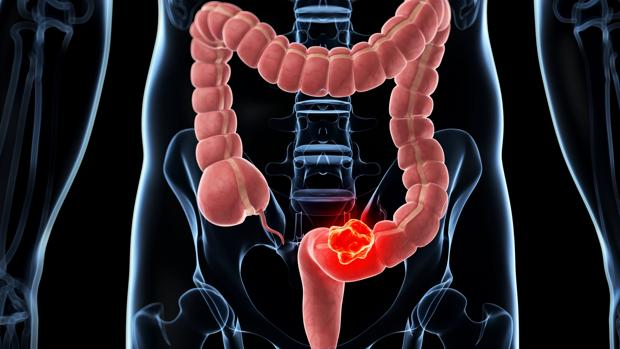
\includegraphics[scale=0.5]{cancer_colon.jpg}
  \caption[Localizaci\'on del c\'ancer colorrectal]{Localizaci\'on del c\'ancer colorrectal \cite{cancer}}
  \label{fig:cancer}
\end{figure}


En la mayoria de los casos de c\'ancer, los factores que est\'an asociados al desarrollo en estas enfermedades tienen una interacci\'on entre s\'i. En el c\'ancer colorrectal, los factores gen\'eticos y ambientales que provocan su desarrollo se favorecen por la interacci\'on de algunos de ellos como el estilo de vida, la dieta y la herencia g\'enetica. En estilos de vida, la falta de ejercicio f\'isico, el sobrepeso y la obesidad, as\'i como el consumo de tabaco y alcohol, son comunes en casos con este tipo de c\'ancer. De manera similar, existe relaci\'on con el consumo de carnes rojas, carne procesada y carne expuesta al fuego directamente, aunque no se ha determinado de que manera los alimentos ricos en fibra, vegetales y leche fungen como protectores ante este tipo de c\'ancer \cite{cancer}. La herencia, representa entre un 20 a un 25\% de los factores de riesgo para esta enfermedad \cite{Riestra}. De manera similar, el c\'ancer colorrectal tiene una prevalencia en individuos mayores a 50 años, siendo esto uno de los mayores riesgos de padecer esta enfermedad. \\



\section{Estructura gen\'etica de la poblaci\'on mexicana}

M\'exico es un pa\'is ubicado en Am\'erica del Norte  y es el tercer pa\'is m\'as grande de Am\'erica Latina. Al d\'ia de hoy, el pa\'is esta conformado por 110 grupo \'etnicos que componen la mayor parte de la poblaci\'on como se muestra en la figura \ref{fig:indigena}. La poblaci\'on de meztizos en M\'exico es de gran proporci\'on seg\'un los datos del \cite{INEGI}. En general, el concepto de \textit{mestizo} en M\'exico es para referirse  personas con una aparencia fenot\'ipica intermedia entre los esterotipos europeos o africanos y tipos de ind\'igenas endemicos del pa\'is \cite{estrada}. \\


\begin{figure}[H]
  \centering
  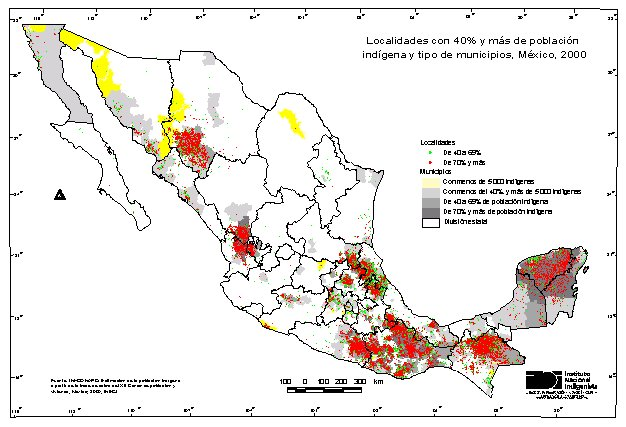
\includegraphics[scale=0.5]{mapa_003.jpg}
  \caption[Mapa de Calor para localidades ind\'igena en M\'exico]{Mapa de calor para localidades con 40\% y m\'as de poblaci\'on ind\'igena en M\'exico. El color rojo muestra las regiones con presencia ind\'igena mayor a 70\% mientras el verde representa la presencia ind\'igena menor al 40\% \cite{CNDPI}}
  \label{fig:indigena}
\end{figure}

La historia de la conquista de M\'exico empez\'o en el año 1559 cuando los europeos, sobre todo españoles, arribaron a las costas de Yucat\'an, empezando el mestizaje en esa zona, añadi\'endose individuos del \'Africa tra\'idos en esclavitud a Am\'erica. Por lo tanto, la mezcla gen\'etica entre los americanos nativos (ind\'igenas), europeos (españoles) y africanos que se produjo en M\'exico form\'o una poblaci\'on mestiza con variadas caracter\'isticas f\'isicas \cite{carlos, Gabriela} como se observa en las siguientes figuras \ref{fig:indi} y \ref{fig:calor}. \\


\begin{figure}[H]
  \centering
  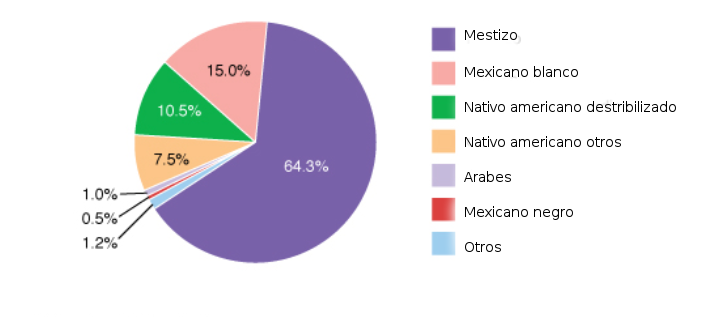
\includegraphics[scale=0.5]{etnia.png}
  \caption[Porcentaje de poblaciones por origen gen\'etico en M\'exico]{Porcentaje de poblaciones por origen gen\'etico en M\'exico \cite{Cat} }
  \label{fig:indi}
\end{figure}


\begin{figure}[H]
  \centering
  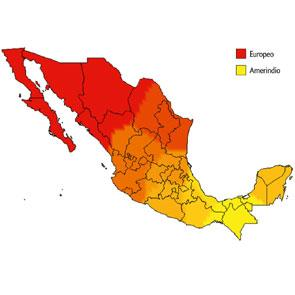
\includegraphics[scale=0.7]{calor_indi.jpg}
  \caption[Mapa de calor de dos poblaciones (europeo y americano nativo)]{Mapa de calor de dos poblaciones con origen gen\'etico europeo y americano nativo \cite{Gabriela}}
  \label{fig:calor}
\end{figure}

\section{Genotipado}\label{sub:geno}

La Academia Europea de Pacientes \cite{ACP} define el genotipado como ``el proceso mediante el cual se determinan las diferencias en los caracteres genéticos o el genotipo de un individuo mediante el análisis de su secuencia de ADN individual. Esto se puede hacer mediante la comparación del genotipo con la secuencia de otro individuo o con una secuencia de referencia''. En otras palabras, el genotipado es la t\'ecnica de laboratorio que se utiliza para determinar la informaci\'on g\'enetica de un organismo, o genotipo, y poder individualizar del resto, as\'i como la susceptibilidad y variantes causales a una enfermedad.\\


Las bases de datos que capturan el genotipado se encuentran en formato \textit{.ped} y \textit{.map} y de un archivo en formato \textit{.xlsx} que muestra los SNPs asociados a la enfermedad. Los archivos .ped describen los individuos y los datos gen\'eticos de la poblaci\'on estudiada. Este archivo puede ser delimitado por \textit{ESPACIOS} o \textit{TAB}, cada l\'inea corresponde a un solo individuo como se puede observar en la siguiente tabla.\\

 \begin{table}[H]
\centering
\begin{tabular}{|1|1|1|1|1|1|1|1|1|1|1|1|1|}
\hline \hline
FAM 1 & IND1 & 0 & 0 & 1 & 0 &  A & A & T & T & 0 & 0 & ...\\
\hline
FAM 2 & IND2 & 0 & 0 & 1 & 0 &  A & G & T & C & T & A & ... \\
\hline
FAM 3 & TRIOF & 0 & 0 & 1 & 0 & A & G & T & C & A & T & ... \\
\hline
FAM 4 & TRIOM & 0 & 0 & 2 & 0 &  A & G & T & C & A & T & ... \\
\hline
FAM 5 & TRIOC & TRIOF & TRIOF & 1 & 0 &  A & A & C & T & A & T & ... \\
\hline \hline
\end{tabular}
\caption{Ejemplo estructura datos .ped}
\label{tabla:ped}
\end{table}

 Las primera seis columnas son: \\

 \begin{enumerate}[1.]
 \item Family ID [\texit{string}]
 \item Individual ID [\texit{string}]
 \item Father ID [\texit{string}]
 \item Mother ID [\texit{string}]
 \item Sex [\texit{integer}]
 \item Phenotype [\texit{float}]
 \end{enumerate}

 Las columnas 7 y 8 codifican los alelos observados en SNP1, las columnas 9 y 10 codifican los alelos observados en SNP2, y así sucesivamente. Los datos faltantes se codifican como "0 0". Este archivo debe tener N líneas y 2L + 6 número de columnas, donde N y L son los números de individuos y SNP contenidos en el conjunto de datos, respectivamente. Es importante resaltar que cada individuo debe tener una identificación única que contenga solo caracteres alfanuméricos.\\

 Por otro lado, el archivo .map describe los SNPs. La estructura de esta informaci\'on se puede observar en la tabla \ref{tabla:map}.\\

 \begin{table}[H]
\centering
\begin{tabular}{|1|1|1|1|}
\hline \hline
7 & SNP1 & 0 & 123\\
\hline
7 & SNP3 & 0 & 456 \\
\hline
7 & SNP3 & 0 & 789\\
\hline \hline
\end{tabular}
\caption{Ejemplo de estructura de datos .map}
\label{tabla:map}
 \end{table}

 De manera similar, este archivo puede estar delimitado por ESPACIOS o TAB. Cada l\'inea corresponde a los SNPs y las cuatro columnas son:\\

 
 \begin{enumerate}[1.]
 \item Chromosome number [\texit{integer}]
 \item SNP ID [\texit{string}]
 \item SNP genetic position (cM) [\texit{float}]
 \item SNP physical position (bp) [\texit{integer}]
 \end{enumerate}


 
 \section{An\'alisis de mezcla de poblaciones}

 El an\'alisis de mezcla de poblaciones se define, seg\'un la International Society of Genetic Genealogy \cite{ISGG}, como un m\'etodo para inferir los or\'igenes geogr\'aficos de alguien basado en un an\'alisis de su ascedencia gen\'etica. La mezcla (Admixture) sucede cuando las poblaciones comienzan con el mestizaje y la desendencia de estas producen una mezcla de alelos de diferentes poblaciones ancestrales. El an\'alisis de este acontecimiento de ancestralidad tiene una importancia valiosa tanto en g\'enetica de poblaciones como en epidemiolog\'ia gen\'etica \cite{Line}.\\

 Esta t\'ecnica tiene como base la clasificaci\'on posible de los individuos en series de grupos \'etnicos com\'unmente identificados tales como europeos, americanos nativos, entre otros. Esto es posible mediante el uso de un SNP informativo de origen ancestral para obtener el porcentaje del genoma de un individuo que tiene un origen ancestral dado \cite{Orlando}, esto se puede observar en la figura \ref{fig:adm}.\\

 
\begin{figure}[H]
  \centering
  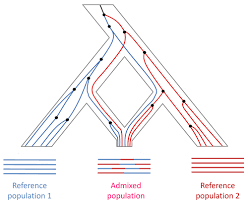
\includegraphics[scale=0.9]{images.png}
  \caption[\'Arbol de poblaci\'on y \'arbol de genes]{ Se observa el \'Arbol de población (en gris) y el árbol de genes (en azul y rojo) que rastrea la historia evolutiva de dos poblaciones ancestrales y su correspondiente población mezclada. Los haplotipos específicos de la población de referencia 1 (líneas rojas) podrían fluir y mezclarse con la población 2 y viceversa  \cite{Yuan}.}
  \label{fig:adm}
\end{figure}
 


\section{Software ADMIXTURE para la estimaci\'on de la ancestralidad}

Varios autores han usado diferentes m\'etodos para la estimaci\'on de ancestr\'ia \cite{Vero,Justo,Nuri}. Los softwares de mayor uso, especificamente diseñados para realizar \textit{admixture mapping} en la literatura son los programas \texttt{STRUCTURE}, \texttt{MALDsoft}, \texttt{ADMIXMAP}, \texttt{ANCESTRYMAP} y \texttt{ADMIXTURE}. Este \'ultimo calcula las estimaciones mucho m\'as r\'apido usando un algoritmo n\'umerico de optimizaci\'on. Especificamente ADMIXTURE es un software para la estimación de máxima verosimilitud de ancestros individuales de conjuntos de datos genotipo SNP multilocus. ADMIXTURE utiliza un enfoque de relajación de bloques (\textbf{block relaxation}, ver el apartado \ref{sec:BR}) para actualizar alternativamente la frecuencia de alelos y los parámetros de la fracción ascendente. Cada actualización de bloques se maneja resolviendo una gran cantidad de problemas de optimización convexos independientes, que se abordan usando un algoritmo de programación cuadrático secuencial rápido. La convergencia del algoritmo se acelera utilizando un novedoso método de aceleración \textit{cuasi Newton} \ref{sec:cn}. El algoritmo supera a los algoritmos EM y los métodos de muestreo MCMC por un amplio margen \cite{Admixture}. Una descripción general de los programas para la estimaci\'on de ancestr\'ia se presenta en la tabla \ref{tabla:sofadm}. \\


\begin{table}[htbp]
  \centering
\begin{tabular}[t]{|1|p{0.3\linewidth}|p{0.4\linewidth}|}
  \hline 
  \multicolumn{1}{|c|}{\textbf{Programa}} & \multicolumn{1}{c|}{\textbf{Global/local}} & \multicolumn{1}{c|}{\textbf{M\'etodo principal}} \tabularnewline \hline
  STRUCTURE & Global/Local & MCMC:Markov Chain Monte Carlo\tabularnewline \hline
frappe &Global&	ML: Maximum likelihood\tabularnewline \hline
ADMIXTURE&Global& EM: Expectation Maximization \tabularnewline \hline
EIGENSTRAT/smartpca&Global&PCA: Principal Component Analysis\tabularnewline \hline
ipPCA/EigenDev&Global&PCA: Principal Component Analysis\tabularnewline \hline
GEMTools&Global& Spectral graph\tabularnewline \hline
PLINK&Global&EM: Expectation Maximization \tabularnewline \hline
LAMP&Local/Global&Hierarchical Hidden Markov Model\tabularnewline \hline
HAPMIX&Local/Global&Infinite hidden Markov model  \tabularnewline \hline
ANCESTRYMAP&Local/Global&Bayesian and ML \tabularnewline \hline

\end{tabular}
\caption[Softwares para la estimaci\'on de ancestr\'ia]{Descripci\'on de softwares  para la estimaci\'on de ancestria local o globlal \cite{Yushi}}
\label{tabla:sofadm}
\end{table}

A grandes rasgos, el software ADMIXTURE estima la probabilidad para los genotipos observados basandose en las proporciones de ascedencia y frecuencias de alelos de poblaci\'on, realiz\'andolo simultaneamente. El archivo de entrada debe de representar a los genotipos de individuos no relacionados, el cual puede ser una estimaci\'on del número de poblaciones \texttt{K}.\\ 

Ahora bien, para la estimaci\'on de la ancestr\'ia ADMIXTURE enfoca sus estimaciones en el m\'etodo de m\'axima verosimilitud (EM) (ver \ref{sec:EM}), en lugar de los m\'etodos tradicionales para estos tipos de estudio como muestrear la distribuci\'on posterior utilizando MCMC. Adem\'as, con el m\'etodo de block relaxation aumenta la velocidad de la estimaci\'on haciendo que sea superior en eficiencia computacional respecto a otros programas de alto nivel como STRUCTURE. En l\'ineas generales, ADMIXTURE actualiza el par\'ametro de frecuencia del alelo y el par\'ametro de fracci\'on ascendente alternativamente maximizando la expansi\'on de la funci\'on de verosimilitud de Taylor de segundo orden. Para realizar este proceso se usa programaci\'on cuadr\'atrica secuencial y se desarrolla de manera iterativa en funci\'on de las frecuencias de los alelos y las proporciones de ascendencia asociadas con los valores de los par\'ametros actuales.Dado que es iterativo y se necesita encontrar un punto \'optimo para resolver $x-M(x) = 0$, el m\'etodo de Newton se puede usar para esta b\'usqueda. Sin embargo, obtener el diferencial de M(x) es desafiante, por lo que se usa un m\'etodo cuasi-Newton, lo que permite la acelaraci\'on de convergencia y tiene una ventaja sobre los m\'etodos de velocidad sobre convergencia como el m\'etodo EM. Se ha probado con datos reales y se ha encontrado que ADMIXTURE es mucho m\'as r\'apido que STRUCTURE pero con una estimaci\'on comparable \cite{Yushi}. \\

Por otro lado, existen dos denominaciones de ADMIXTURE para estimar la ancestr\'ia. La estimaci\'on de ascedencia se demonina \textbf{Supervisada} cuando se considera los genotipos de individuos con ancestros conocidos, para ello se necesita archivos \texttt{.pop}. Cuando no se incluyen individuos con ancestros conocidos entonces se denomina \txtbf{no supervisada} \cite{Timothy}.\\


\section{Estimaci\'on de ancestr\'ia por proyecci\'on}

Cuando se tiene un conjunto de datos nuevo de genes, donde se tiene como
objetivo estimar la ancestria, existe la manera de utilizar conjuntos
de datos como paneles de referencia, tales como los proyectos
\textbf{1000Genomes} o \textbf{HapMap}. Estos se usan en combinaci\'on con la
muestra del estudio para estimación de la ancestr\'ia utilizando softwares como ADMIXTURE, debido a que estos grandes conjuntos de
datos resumen la estructura de la poblaci\'on humana. Es decir, para
las muestras del estudio que no incluyen una poblaci\'on nueva, una
forma eficiente de estimar la ascedencia individual es
\textbf{proyectar} las nuevas muestras en la estructura de la poblaci\'on conocida (aprendida) de los paneles de referencia.\\

La manera en que se realiza esta operaci\'on tiene una estructura similar a la operaci\'on de proyecci\'on utilizada en el an\'alisis de componentes principales, aunque los detalles matem\'aticos difieren. Para el tipo de poyecci\'on no supervisada se requiere que las dos bases de datos (los paneles de referencia y los datos del estudio) tengan los mismos SNP's, siendo que se aprende del conjunto de datos de referencia y las proporciones de ascendencia se pueden inferir para el conjunto de datos del estudio.\\

En el aspecto matem\'atico, esto requiere resolver el problema de maximizaci\'on de verosimilitud de la ecuaci\'on 4.2, del capitulo 4, con respecto a \texttt{Q} para un \texttt{P} fijo. Este tipo de problemas son convexos y se resuelven de manera eficiente con la ayuda de los algoritmos de optimizaci\'on como Block Relaxation \cite{Suyash}.



%%%%%%%%%%%%%%%%%%%%%%%%%%%%%%%%%%%%%%%%%%%%%%%%%%%%%%%%%%%%%%%%%%%%%%%%%%%%%%%%%%%%%%%%%%%%%%%%%%%%%%%%%%%%%%%%%%%%%%%%%%%%%%%%%%%%%%%%%%%%%% %%%%%%%%%%%%%%%%%%%%%%%%%%%%%%%%%%%%%%%%%%%%%%%%%%%%%%%%%%%%%%%%%%%%%%%%%%%%%%%%%%%%%%%%%%%%%%%%


